\documentclass{book}
\usepackage{graphicx}
\usepackage[final]{pdfpages}


\begin{document}

\chapter{Appendices}

\section{Key terms}
	\begin{itemize}
		\item 	Repeatability - variability in returning to the same previously taught position/configuration
		\item Accuracy - variability in moving to a target in space that has not been previously taught
		\item Tool speed - linear speed capability when tool moving along a curvilinear path
		\item Screw speed - rotational speed when tool is being rotated about an axis in space
		\item Joint interpolated motion - motion where joint taking longest time to make the joint change governs the motion and the other joints are slowed in proportion so that all joints accomplish their joint changes simultaneously with the slowest joint
		\item Joint limits - either the software or physical hardware limits which constrain the operating range of a joint on a robot. The software limits have a smaller range than the hardware limits.
		\item Joint speed limits - speed limit for robot joints, which limit how fast the links of a robot may translate or rotate.
		\item Point-to-point motion - characterized by starting and stopping between configurations or as the tool is moved between targets.
		\item Continuous path motion - characterized by blending of motion between configurations or targets, usually with the loss of path accuracy at the target transitions, as the robot moves between configurations/targets.
		\item Interpolation (kinematic) capabilities - robot usually capable of both forward and inverse kinematics. Both combine to give the robot the capability to move in joint space and in  Cartesian space. We typically refer to the moves as joint, linear, or circular interpolation.
		\item Forward kinematics - specifying the joint values to accomplish a robot move to a new configuration in space. These may not be simple as it seems because secondary joints such as four-bar linkages, ball screws, etc. may be required to accomplish this motion.
		\item Inverse kinematics - solving a mathematical model of the robot kinematics to determine the necessary joint values to move the tool to a desired target (frame) in space. This is accomplished by frame representation whereby a triad (xyz axes) is attached to the tool on the robot and a target frame is attached to the part or operating point in the workcell. The inverse kinematics determine the joint values that align the tool triad with the target triad.
		\item I/O - input/output which consist of ON/OFF signal values, threshold values, or analog signal values which allow the control of or response to external devices/sensors as required to sequence workcell operations.
		\item Programming language - The language and logical constructs used to program the set of operational instructions used to control robot movement and interact with sensors and other cell devices.
		\item Multi-tasking - ability to process more than one program at a time or process I/O concurrently.
		\item Load capability - force and torque capability of the robot at its tool interface
		\item TCF - tool or terminal control frame
		\item TCP - tool/terminal control point
		\item Teach Pendant - Operator interface device used to teach/save robot \item configurations and program simple instructions.
	\end{itemize}

\newpage
	\section{Kinect specifications}
		\begin{center}
		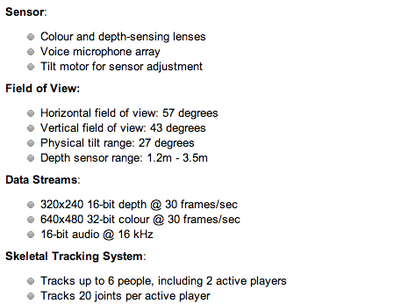
\includegraphics[scale=1]{kinect1}	
		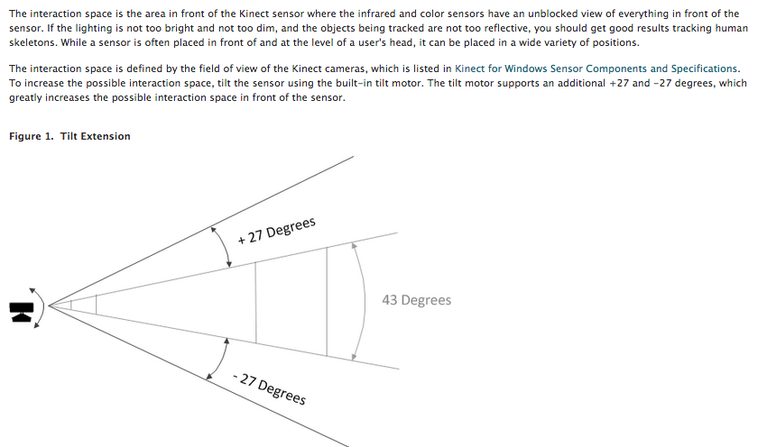
\includegraphics[scale=1]{kinect2}
		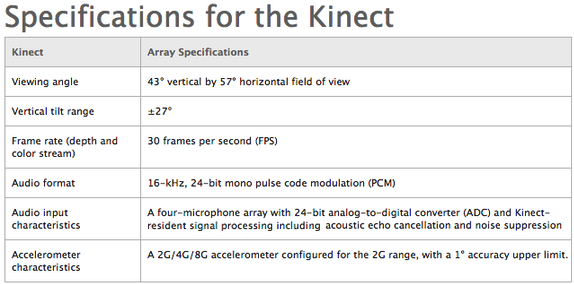
\includegraphics[scale=1]{kinect3}
		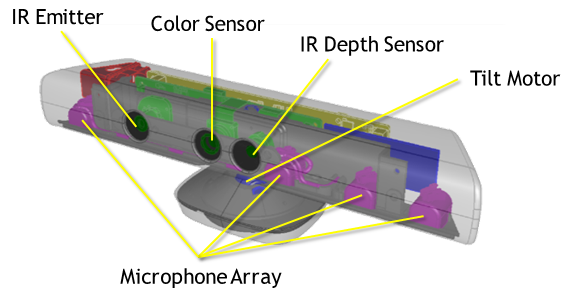
\includegraphics[scale=0.8]{kinect4}
	\end{center}
	
	\newpage

		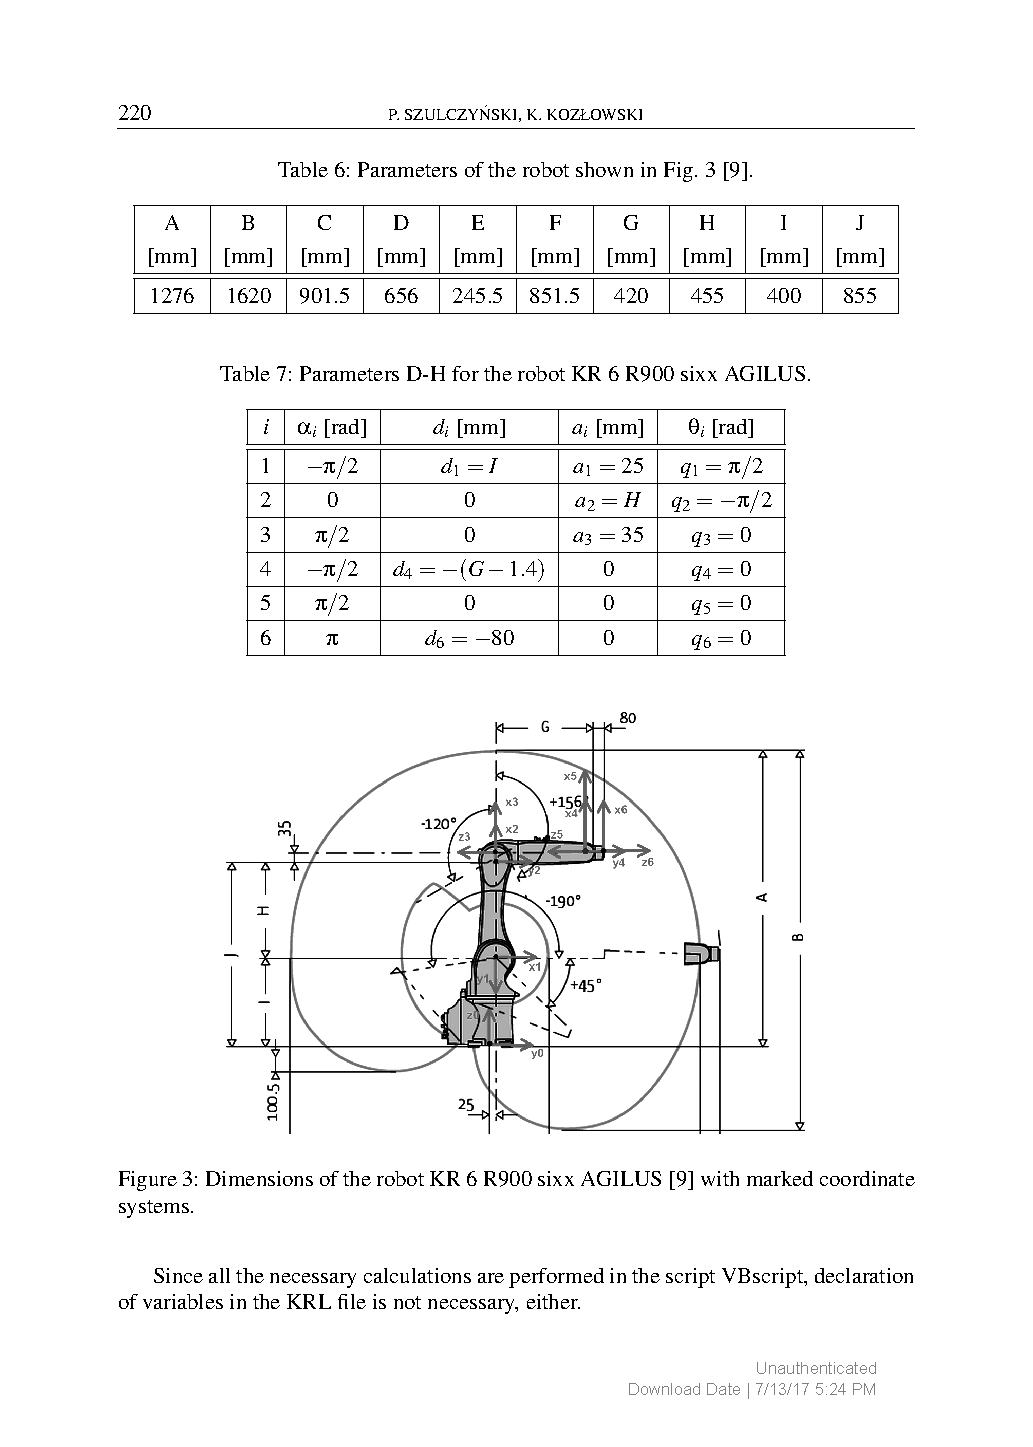
\includepdf[pages=1]{appendix.pdf}

		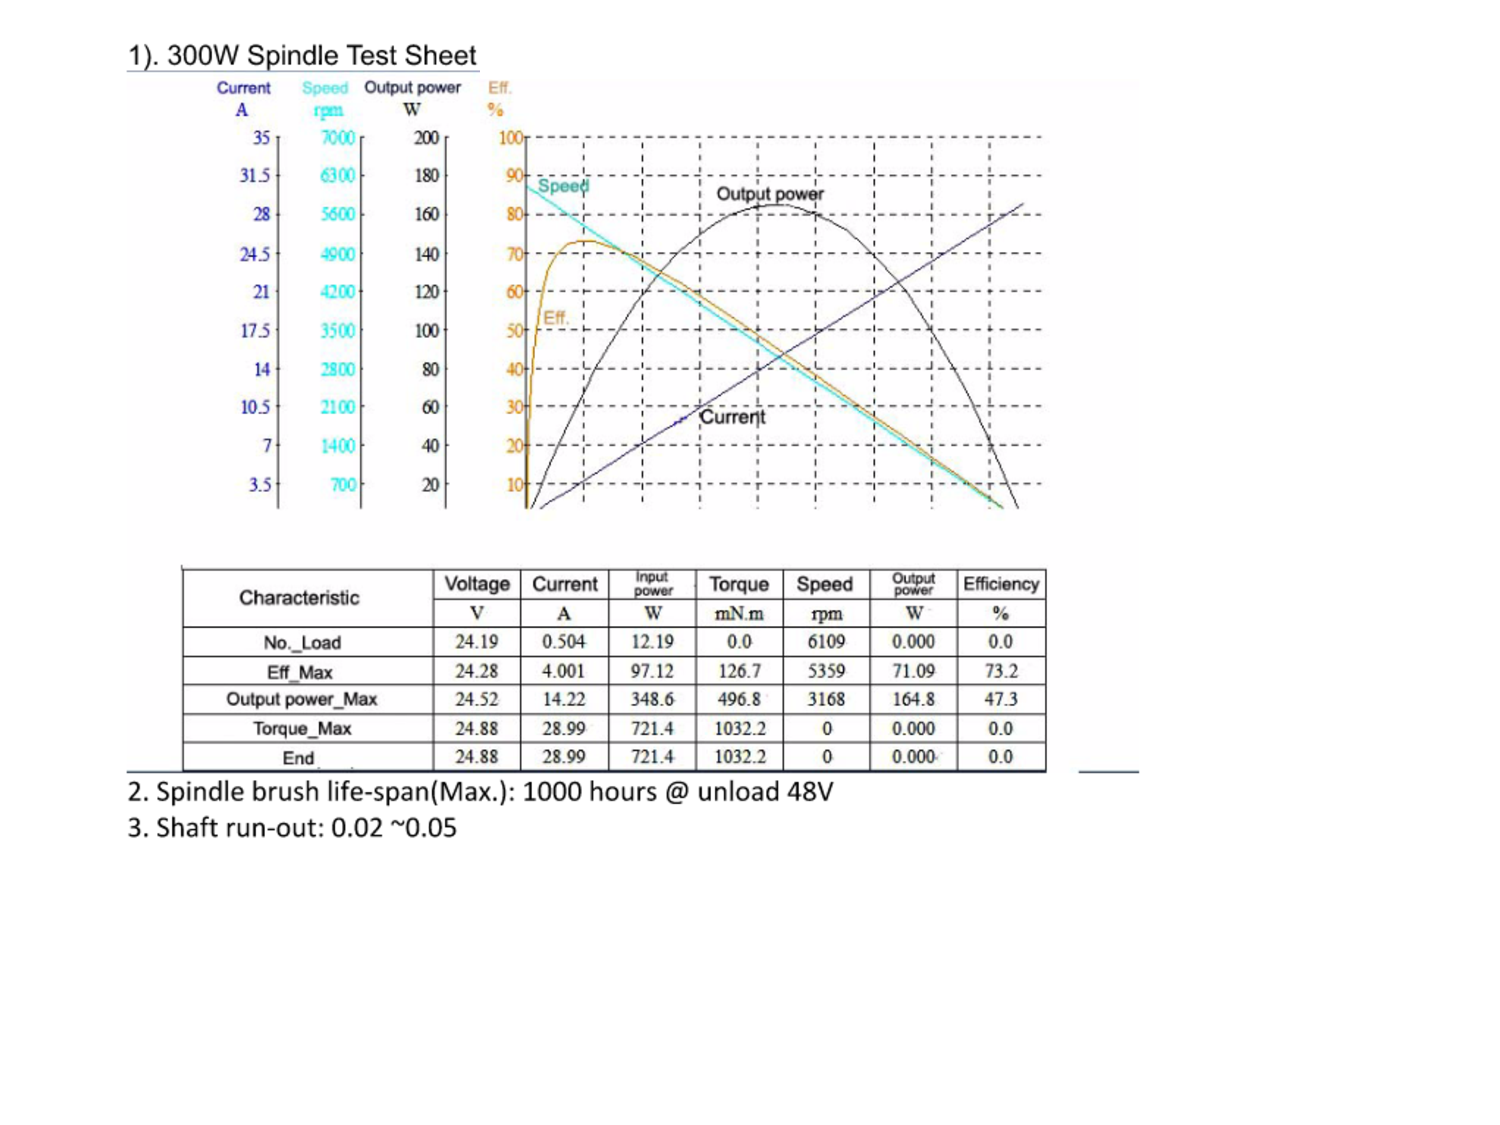
\includepdf[pages=1]{spindle.pdf}

	\newpage
	\section{Codes}
		\subsection{KUKAVARPROXY.py}
		\begin{verbatim}
		
		import socket                                                   # Used for TCP/IP communication
		client = socket.socket(socket.AF_INET, socket.SOCK_STREAM)		# Initializing client connection
		
		class KUKA(object):
		
		def __init__(self, TCP_IP):
		try: 
		client.connect((TCP_IP, 7000))                      # Open socket. kukavarproxy actively listens on TCP port 7000
		except: 
		self.error_list(1)
		
		
		def send (self, var, val, msgID):
		"""
		kukavarproxy message format is 
		msg ID in HEX                       2 bytes
		msg length in HEX                   2 bytes
		read (0) or write (1)               1 byte
		variable name length in HEX         2 bytes
		variable name in ASCII              # bytes
		variable value length in HEX        2 bytes
		variable value in ASCII             # bytes
		"""
		try:
		msg = bytearray()
		temp = bytearray()
		if val != "":
		val = str(val)
		msg.append((len(val) & 0xff00) >> 8)            # MSB of variable value length
		msg.append((len(val) & 0x00ff))                 # LSB of variable value length
		msg.extend(map(ord, val))                       # Variable value in ASCII
		temp.append(bool(val))                              # Read (0) or Write (1)
		temp.append(((len(var)) & 0xff00) >> 8)             # MSB of variable name length
		temp.append((len(var)) & 0x00ff)                    # LSB of variable name length
		temp.extend(map(ord, var))                          # Variable name in ASCII 
		msg = temp + msg
		del temp[:]
		temp.append((msgID & 0xff00) >> 8)                  # MSB of message ID
		temp.append(msgID & 0x00ff)                         # LSB of message ID
		temp.append((len(msg) & 0xff00) >> 8)               # MSB of message length
		temp.append((len(msg) & 0x00ff))                    # LSB of message length
		msg = temp + msg
		except :
		self.error_list(2)
		try:
		client.send(msg)
		return  client.recv(1024)                           # Return response with buffer size of 1024 bytes
		except :
		self.error_list(1)
		
		
		def __get_var(self, msg):
		"""
		kukavarproxy response format is 
		msg ID in HEX                       2 bytes
		msg length in HEX                   2 bytes
		read (0) or write (1)               1 byte
		variable value length in HEX        2 bytes
		variable value in ASCII             # bytes
		Not sure if the following bytes contain the client number, or they're just check bytes. I'll check later.
		"""
		try:
		# Python 2.x
		lsb = (int (str(msg[5]).encode('hex'),16))
		msb = (int (str(msg[6]).encode('hex'),16))
		lenValue = (lsb <<8 | msb)
		return msg [7: 7+lenValue]
		
		"""
		# Python 3.x
		lsb = int( msg[5])
		msb = int( msg[6])
		lenValue = (lsb <<8 | msb)
		return str(msg [7: 7+lenValue],'utf-8')  
		"""
		
		except:
		self.error_list(2)
		
		def read (self, var, msgID=0):
		try:
		return self.__get_var(self.send(var,"",msgID))  
		except :
		self.error_list(2)
		
		
		def write (self, var, val, msgID=0):
		try:
		if val != (""): return self.__get_var(self.send(var,val,msgID))
		else: raise self.error_list(3)
		except :
		self.error_list(2)
		
		
		def disconnect (self):
		client.close()                                      # CLose socket
		
		
		def error_list (self, ID):
		if ID == 1:
		print ("Network Error (tcp_error)")
		print ("    Check your KRC's IP address on the network, and make sure kukaproxyvar is running.")
		self.disconnect()
		raise SystemExit
		elif ID == 2:
		print ("Python Error.")
		print ("    Check the code and uncomment the lines related to your python version.")
		self.disconnect()
		raise SystemExit
		elif ID == 3:
		print ("Error in write() statement.")
		print ("    Variable value is not defined.")
	\end{verbatim}


	\newpage
	\subsection{KRLDRIVER.SRC}
	
	\begin{verbatim}
	
		&ACCESS RVP
		&REL 8
		&PARAM EDITMASK = *
		&PARAM TEMPLATE = C:\KRC\Roboter\Template\vorgabe
		DEF KRLDRIVER( )
		;FOLD INI;%{PE}
		;FOLD BASISTECH INI
		GLOBAL INTERRUPT DECL 3 WHEN $STOPMESS==TRUE DO IR_STOPM ( )
		INTERRUPT ON 3 
		BAS (#INITMOV,0 )
		;ENDFOLD (BASISTECH INI)
		;FOLD SPOTTECH INI
		USERSPOT(#INIT)
		;ENDFOLD (SPOTTECH INI)
		;FOLD GRIPPERTECH INI
		USER_GRP(0,DUMMY,DUMMY,GDEFAULT)
		;ENDFOLD (GRIPPERTECH INI)
		;FOLD USER INI
		;Make your modifications here
		
		;ENDFOLD (USER INI)
		;ENDFOLD (INI)
		KRLD_COM=0
		$ADVANCE=1
		$PAL_MODE=FALSE
		$OV_PRO=100
		PTP {A1 0, A2 -90, A3 90, A4 0, A5 0, A6 0}
		WHILE TRUE
		SWITCH KRLD_COM
		CASE 1
		KRLD_COM=0
		PTP KRLD_AXIS C_PTP
		
		CASE 2
		KRLD_COM=0
		PTP KRLD_POS C_PTP
		
		CASE 3
		KRLD_COM=0
		LIN KRLD_POS C_DIS
		
		CASE 4
		KRLD_COM=0
		CIRC KRLD_POS_AUX, KRLD_POS
		
		CASE 5
		KRLD_COM=0
		PTP_REL KRLD_AXIS C_PTP
		
		CASE 6
		KRLD_COM=0
		PTP_REL KRLD_POS C_PTP
		
		CASE 7
		KRLD_COM=0
		LIN_REL KRLD_POS C_DIS
		
		CASE 8
		KRLD_COM=0
		WAIT SEC KRLD_SLEEP
		
		CASE 9
		KRLD_COM=0
		$BASE=KRLD_BASE:KRLD_BASE_OFFSET
		
		CASE 10
		KRLD_COM=0
		$TOOL=KRLD_TOOL
		
		CASE 11
		KRLD_COM=0
		$APO.CPTP=KRLD_APO
		$APO.CDIS=KRLD_APO
		
		CASE 12
		KRLD_COM=0
		$VEL.CP=KRLD_VEL_CP
		
		CASE 13
		KRLD_COM=0
		BAS(#VEL_PTP,KRLD_VEL_PTP) 
		
		CASE 14
		KRLD_COM=0
		$OUT[KRLD_IO]=KRLD_SIGNAL
		
		CASE 15
		KRLD_COM=0
		$PAL_MODE= KRLD_SIGNAL
		ENDSWITCH
		ENDWHILE
		END
	\end{verbatim}

	\newpage
	\subsection{KRLDRIVER.py}
	\begin{verbatim}
	
		from kukavarproxy import *
		
		robot = KUKA('172.31.1.147')
		
		axes_limits = [ [-170,170],[-190,45],[-120,156],[-185,185],[-120,120],[-350,350]]
		AXIS = 'a'
		POS = 'p'
		FALSE = 0
		TRUE = 1
		
		def INI(VEL_CP_VAL=3, VEL_AXIS_VAL=100, OV_PRO_VAL=10 ,APO_VAL=0):
		VEL_CP(VEL_CP_VAL)
		VEL_PTP(VEL_AXIS_VAL)
		OV_PRO(OV_PRO_VAL)
		APO(APO_VAL)
		BASE(525,0,890,0,0,0)
		TOOL(0,0,0,0,-90,0) 
		PTP(POS,0,0,0,0,0,0)
		
		def PTP_HOME():
		PTP(AXIS,0,-90,90,0,0,0)
		
		def GRIPPER_OPEN():
		OUT(1,TRUE)
		OUT(1,FALSE)
		OUT(4,TRUE)
		OUT(4,FALSE)
		
		def GRIPPER_CLOSE():
		OUT(4,TRUE)
		OUT(4,FALSE)
		OUT(1,TRUE)
		OUT(1,FALSE)
		
		def OUT(ioPort, Signal):
		while (int (robot.read("KRLD_COM"))): continue
		robot.write("KRLD_IO",ioPort)
		if Signal == True: robot.write("KRLD_SIGNAL","TRUE")
		else: robot.write("KRLD_SIGNAL","FALSE")
		robot.write("KRLD_COM",14)
		
		def PAL_MODE(Signal):
		while (int (robot.read("KRLD_COM"))): continue
		if Signal == True: robot.write("KRLD_SIGNAL","TRUE")
		else: robot.write("KRLD_SIGNAL","FALSE")
		robot.write("KRLD_COM",15)
		
		def PTP(interpolation, v1="",v2="",v3="",v4="",v5="",v6=""):
		if v1 == v2 == v3 == v4 == v5 == v6 == "": 
		raise error(2)
		return 0
		if interpolation == AXIS: 
		axes = [v1,v2,v3,v4,v5,v5]
		for index,axis in enumerate(axes):
		pass
		#if float(axis) <= axes_limits[index][0] or float(axis) >= axes_limits[index][1]: raise error(1,(index+1))
		while (int (robot.read("KRLD_COM"))): continue
		destination = format_axis(v1,v2,v3,v4,v5,v6)
		robot.write("KRLD_AXIS", destination)
		robot.write("KRLD_COM",1)
		elif interpolation == POS:
		while (int (robot.read("KRLD_COM"))): continue
		destination = format_pos(v1,v2,v3,v4,v5,v6)
		robot.write("KRLD_POS",destination)
		robot.write("KRLD_COM",2)
		else:
		raise error(3)
		
		def PTP_REL(interpolation, v1="",v2="",v3="",v4="",v5="",v6=""):
		if v1 == v2 == v3 == v4 == v5 == v6 == "": 
		raise error(2)
		return 0
		if interpolation == AXIS: 
		while (int (robot.read("KRLD_COM"))): continue
		destination = format_axis(v1,v2,v3,v4,v5,v6)
		robot.write("KRLD_AXIS", destination)
		robot.write("KRLD_COM",5)
		elif interpolation == POS:
		while (int (robot.read("KRLD_COM"))): continue
		destination = format_pos(v1,v2,v3,v4,v5,v6)
		robot.write("KRLD_POS",destination)
		robot.write("KRLD_COM",6)
		else:
		raise error(3)
		
		def LIN (x="",y="",z="",a="",b="",c=""):
		if x == y == z == a == b == c == "": raise error(3)
		while (int (robot.read("KRLD_COM"))): continue
		destination = format_pos(x,y,z,a,b,c)
		robot.write("KRLD_POS",destination)
		robot.write("KRLD_COM",3)
		
		def LIN_REL (x="",y="",z="",a="",b="",c=""):
		if x == y == z == a == b == c == "": raise error(3)
		while (int (robot.read("KRLD_COM"))): continue
		destination = format_pos(x,y,z,a,b,c)
		robot.write("KRLD_POS",destination)
		robot.write("KRLD_COM",7)
		
		def CIRC (x="",y="",z="",a="",b="",c="",xAux="",yAux="",zAux="",aAux="",bAux="",cAux=""):
		if x == y == z == a == b == c == "": raise error(3)
		if xAux == yAux == zAux == aAux == bAux == cAux == "": raise error(5)
		while (int (robot.read("KRLD_COM"))): continue
		destination = format_pos(x,y,z,a,b,c)
		robot.write("KRLD_POS",destination)
		auxilliary = format_pos(xAux,yAux,zAux,aAux,bAux,cAux)
		robot.write("KRLD_POS",auxilliary)
		robot.write("KRLD_COM",4)
		
		def WAIT(time_sec):
		while (int (robot.read("KRLD_COM"))): continue
		robot.write("KRLD_SLEEP", abs(time_sec))
		robot.write("KRLD_COM",8)
		
		def BASE(x=0,y=0,z=0,a=0,b=0,c=0,offX=0,offY=0,offZ=0,offA=0,offB=0,offC=0,BASE_DATA=-1):
		while (int (robot.read("KRLD_COM"))): continue
		if BASE_DATA > 0: 
		base_frame = "BASE_DATA["  + str(BASE_DATA) + "]"
		robot.write("KRLD_BASE", robot.read(base_frame))	
		else:
		if x == y == z == a == b == c == "": raise error(3)
		base_frame = format_pos(x,y,z,a,b,c)
		robot.write("KRLD_BASE", base_frame)
		offset_data = format_pos(offX,offY,offZ,offA,offB,offC)
		robot.write("KRLD_BASE_OFFSET", offset_data)
		robot.write("KRLD_COM",9)
		
		def TOOL(x=0,y=0,z=0,a=0,b=0,c=0,TOOL_DATA=-1):
		while (int (robot.read("KRLD_COM"))): continue
		if TOOL_DATA > 0: 
		tool_frame = "TOOL_DATA["  + str(TOOL_DATA) + "]" 
		robot.write("KRLD_TOOL", robot.read(tool_frame))
		else:
		if x == y == z == a == b == c == "": raise error(3)
		tool_frame = format_pos(x,y,z,a,b,c)
		robot.write("KRLD_TOOL", tool_frame)
		robot.write("KRLD_COM",10)
		
		def APO(approximation_value):
		while (int (robot.read("KRLD_COM"))): continue
		robot.write("KRLD_APO", approximation_value )
		robot.write("KRLD_COM",11)
		
		def VEL_CP(velocity_value):
		while (int (robot.read("KRLD_COM"))): continue
		robot.write("KRLD_VEL_CP", velocity_value)
		robot.write("KRLD_COM",12)
		
		def VEL_PTP(velocity_value):
		while (int (robot.read("KRLD_COM"))): continue
		robot.write("KRLD_VEL_PTP", velocity_value)
		robot.write("KRLD_COM",13)
		
		def OV_PRO(percentage):
		while (int (robot.read("KRLD_COM"))): continue
		if percentage < 0 or percentage > 100: raise error(4)
		robot.write("$OV_PRO", percentage)
		
		
		def format_axis(A1, A2, A3, A4, A5, A6):
		axes = [A1,A2,A3,A4,A5,A6]
		axes_names = ["A1","A2","A3","A4","A5","A6"]
		instruction = " "
		for index,axis in enumerate(axes):
		if axis != "":
		if instruction[len(instruction)-1] != " ":	instruction += ", "
		instruction += axes_names[index] + " " + str(axis)
		return "{" + instruction + "}"
		
		def format_pos(x, y, z, a, b, c):
		coordinates = [x,y,z,a,b,c]
		coordinates_names = ["X","Y","Z","A","B","C"]
		instruction = " "
		for index,coordinate in enumerate(coordinates):
		if coordinate != "":
		if instruction[len(instruction)-1] != " ":	instruction += ", "
		instruction += coordinates_names[index] + " " + str(coordinate)
		return "{" + instruction + "}"
		
		def error(index, axis=9):
		if index == 1: print("A" + str(axis)+ " limits violated.")
		if index == 2: print("One parameter- at least- should be defined for motion.")
		if index == 3: print("Interpolation type is wrongly defined.")
		if index == 4: print("$OV_PRO values should be percentage.")
		if index == 5: print("Incorrect base number.")
		if index == 6: print("One auxilliary coordinate- at least- should be defined for CIRC motion.")
		raise SystemExit
		\end{verbatim}
	
	\newpage
	\subsection{zukaHandGuiding.py}
	\begin{verbatim}
	
		#!/usr/bin/env python
		import rospy
		import roslib
		import tf
		import time
		from math import *
		from krldriver import *
		
		def main():	
		PAL_MODE(TRUE)
		VEL_CP(3)
		VEL_PTP(100)
		OV_PRO(10)
		APO(30)
		BASE(750,0,770,0,0,0)
		TOOL(0,0,0,0,-90,0) 	
		
		rospy.init_node('ZUKA_Hand_Guiding', anonymous=True)
		print("Node Initialized.")
		listener = tf.TransformListener()
		running = False
		notificationSent = False
		user = 1
		gripState = False
		
		xcalib = 0
		ycalib = 0
		zcalib = 0
		wcalib = 0
		
		xRobot = 0
		yRobot = 0
		zRobot = 0
		wRobot = 0
		
		
		while not rospy.is_shutdown():
		readings = 0
		xlist = []
		ylist = []
		zlist = []
		wlist = []
		zKick = []
		yKick = []
		
		while readings < 50:
		try:	
		listener.waitForTransform("/torso_%d" %user,"/left_hand_%d" %user, rospy.Time(), rospy.Duration(1))
		trans, rot = listener.lookupTransform("/torso_%d" %user, "/left_hand_%d" %user, rospy.Time())
		xlist += [trans[0]*1000]
		ylist += [trans[1]*1000]
		zlist += [trans[2]*1000]
		
		listener.waitForTransform("/openni_depth_frame", "/torso_%d" %user, rospy.Time(), rospy.Duration(1))
		trans, rot = listener.lookupTransform("/openni_depth_frame", "/torso_%d" %user, rospy.Time())
		if rot[3] > 0: wlist += [rot[3]*5*180.0/pi]
		else : wlist += [rot[3]*4.2*180.0/pi]
		
		listener.waitForTransform("/torso_%d" %user,"/right_hand_%d" %user, rospy.Time(), rospy.Duration(1))
		trans, rot = listener.lookupTransform("/torso_%d" %user, "/right_hand_%d" %user, rospy.Time())
		zKick += [trans[2]*1000]
		yKick += [trans[1]*1000]
		readings += 1
		except (tf.LookupException, tf.ConnectivityException, tf.ExtrapolationException,tf.Exception) :
		if rospy.is_shutdown(): return
		user = user + 1
		if user > 5 : user = 1
		print "Trying user", user
		notificationSent = False
		running = False
		
		x = int(sum(xlist))/len(xlist)
		y = int(sum(ylist))/len(ylist)
		z = int(sum(zlist))/len(zlist)
		w = int(sum(wlist))/len(wlist)
		zKick = int(sum(zKick))/len(zKick)
		yKick = int(sum(yKick))/len(yKick)
		
		
		# HERE GOES THE ALGORITHM
		if (zKick) < (-350) and yKick > 100 and not running:
		for i in range(5):
		print ("Starting in %d" %(5-i))
		time.sleep(1)
		if rospy.is_shutdown(): return
		wcalib = 0
		running = True	
		print ("Tracking...")
		continue
		
		elif (zKick) < (-350) and yKick > 100 and running:
		print ("Tracking has stopped")
		running = False
		notificationSent = False
		time.sleep(2)
		rospy.signal_shutdown("User Kick detected.")
		
		elif (zKick) < (-150) and yKick < 0 and running:
		if gripState == False: 
		GRIPPER_OPEN()
		gripState = True
		else: 
		GRIPPER_CLOSE()
		gripState = False
		time.sleep(.5)	
		
		elif running:
		wRel = w - wcalib
		yRel = y - ycalib
		zRel = z - zcalib
		if wcalib == 0: 
		wcalib = w
		ycalib = y
		zcalib = z
		else: 
		# The code 
		if abs(wRel - wRobot) > 2:
		wRobot = max(min(169, wRel), (-169))
		#print wRobot , yRel, zRel
		BASE(350,0,750,0,0,0,0,0,0,(-wRobot))	
		PTP(POS,-zRel,0,yRel,"",0,0)
		#print yKick, zKick	
		time.sleep(.01)
		else:
		if not notificationSent:
		print ("User %d is active. Waiting for the kick."% user)	
		notificationSent = True
		
		
		
		
		
		if __name__ == "__main__":
		main()
	\end{verbatim}

	\newpage
	\subsection{zukaSafeOperation}
	\begin{verbatim}
		#!/usr/bin/env python
		import os
		import threading
		import rospy
		from std_msgs.msg import Float32
		from kukavarproxy import *
		
		zuka = KUKA('172.31.1.148')
		
		safeRange = 1500
		limitedSpeed = 0
		fullSpeed = int (zuka.read("$OV_PRO"))
		
		
		speedChanged = False
		
		def openniTracker():
		global speedChanged
		while 1:
		print" LOW SPEED"
		speedChanged = True
		zuka.write("$OV_PRO",limitedSpeed)
		os.system("killall -9 openni_tracker")
		print"Loading Openni Tracker ..."
		os.system("rosrun openni_tracker openni_tracker")
		
		def get_distance(distance):
		global speedChanged
		if distance.data < safeRange and not speedChanged:
		print" LOW SPEED"
		zuka.write("$OV_PRO",limitedSpeed)
		speedChanged = True
		
		if distance.data > safeRange and speedChanged:
		print" FULL SPEED"
		zuka.write("$OV_PRO",fullSpeed)
		speedChanged = False
		
		def main():	
		lol= rospy.Subscriber("/closestUser", Float32, get_distance)
		rospy.init_node('zukaSafeOperation', anonymous=True)
		
		t = threading.Thread(target = openniTracker,args = ())
		t.start()
		
		while not rospy.is_shutdown():
		if lol.get_num_connections() == 0 : 
		lol.unregister()
		lol= rospy.Subscriber("/closestUser", Float32, get_distance)
		
		
		if \__name\__ == "\__main\__":
		main()
	\end{verbatim}


\end{document}
